
%%%%%%%% ICML 2018 EXAMPLE LATEX SUBMISSION FILE %%%%%%%%%%%%%%%%%

\documentclass{article}

% Recommended, but optional, packages for figures and better typesetting:
\usepackage{microtype}
\usepackage{graphicx}
%\usepackage{subfigure}
\usepackage{booktabs} % for professional tables

% hyperref makes hyperlinks in the resulting PDF.
% If your build breaks (sometimes temporarily if a hyperlink spans a page)
% please comment out the following usepackage line and replace
% \usepackage{icml2018} with \usepackage[nohyperref]{icml2018} above.
%\usepackage{hyperref}

% Attempt to make hyperref and algorithmic work together better:
\newcommand{\theHalgorithm}{\arabic{algorithm}}

\newcommand{\system}{\textsc{DreamCoder}~}
\newcommand{\systemEnding}{\textsc{DreamCoder}}
\newcommand{\lowerBound}{\mathscr{L}}
\newcommand{\code}[1]{{\footnotesize\texttt{#1}}}
\newcommand{\codechar}[1]{{\footnotesize{\texttt{"#1"}}}}
% Use the following line for the initial blind version submitted for review:
\usepackage[nohyperref]{icml2018}

\usepackage{xcolor}
\definecolor{pop1}{HTML}{1f78b4}
\definecolor{pop2}{HTML}{297F23}
\definecolor{pop3}{HTML}{d95f02}
\definecolor{orange}{HTML}{d95f02}
\definecolor{teal}{HTML}{1b9e77}
\newcommand{\pop}[1]{\textcolor{pop1}{#1}}
\newcommand{\popp}[1]{\textcolor{pop2}{#1}}
\newcommand{\tree}[1]{\textcolor{pop3}{#1}}
\newcommand{\orange}[1]{\textcolor{orange}{#1}}
\newcommand{\teal}[1]{\textcolor{teal}{#1}}


%\usepackage{hyperref}       % hyperlinks
\usepackage{url}            % simple URL typesetting
\usepackage{booktabs}       % professional-quality tables
\usepackage{amsfonts}       % blackboard math symbols
\usepackage{nicefrac}       % compact symbols for 1/2, etc.
\usepackage{microtype}      % microtypography
\usepackage{mathrsfs}
\usepackage{listings}
\usepackage{amsthm}
% use Times
\usepackage{times}
% For figures
\usepackage{graphicx} % more modern
%\usepackage{epsfig} % less modern
\usepackage{subfig} 
\usepackage{fancyvrb}


\usepackage{caption}
%\usepackage{subcaption}

\fvset{fontsize=\footnotesize}

\usepackage{amssymb}
\usepackage{listings}
\usepackage{wrapfig}
\usepackage{tabularx}


\usepackage{verbatim}
 \usepackage{booktabs}
 % For algorithms
\usepackage{algorithm}
\usepackage{algorithmic}
\usepackage{tikz}
\usepackage{circuitikz}
\usetikzlibrary{fit,bayesnet}
%\usetikzlibrary{arrows.meta}
%\usetikzlibrary{positioning}
%\usetikzlibrary{decorations.text}
%\usetikzlibrary{decorations.pathmorphing}
\usepackage{dsfont}
\usepackage{amsmath}

\DeclareMathOperator*{\argmin}{arg\,min} % thin space, limits underneath in displays
\DeclareMathOperator*{\argmax}{arg\,max} % thin space, limits underneath in displays
 


% Packages hyperref and algorithmic misbehave sometimes.  We can fix
% this with the following command.

\newcommand{\Expect}{\mathds{E}} %{{\rm I\kern-.3em E}}
\newcommand{\indicator}{\mathds{1}} %{{\rm I\kern-.3em E}}
\newcommand{\expect}{\mathds{E}} %{{\rm I\kern-.3em E}}
\newcommand{\probability}{\mathds{P}} %{{\rm I\kern-.3em P}}



% If accepted, instead use the following line for the camera-ready submission:
%\usepackage[accepted]{icml2018}

% The \icmltitle you define below is probably too long as a header.
% Therefore, a short form for the running title is supplied here:
\icmltitlerunning{Bootstrapping Domain-Specific Languages for Neurally-Guided Bayesian Program Learning}

\begin{document}

\twocolumn[
\icmltitle{\systemEnding: Bootstrapping Domain-Specific Languages for Neurally-Guided Bayesian Program Learning}

% It is OKAY to include author information, even for blind
% submissions: the style file will automatically remove it for you
% unless you've provided the [accepted] option to the icml2018
% package.

% List of affiliations: The first argument should be a (short)
% identifier you will use later to specify author affiliations
% Academic affiliations should list Department, University, City, Region, Country
% Industry affiliations should list Company, City, Region, Country

% You can specify symbols, otherwise they are numbered in order.
% Ideally, you should not use this facility. Affiliations will be numbered
% in order of appearance and this is the preferred way.
\icmlsetsymbol{equal}{*}

\begin{icmlauthorlist}
\icmlauthor{Kevin Ellis}{MIT}
\icmlauthor{Lucas Morales}{MIT}
\icmlauthor{Matthias}{MIT}
\icmlauthor{Armando Solar-Lezama}{MIT}
\icmlauthor{Joshua B. Tenenbaum}{MIT}
\end{icmlauthorlist}

%\icmlaffiliation{to}{Department of Computation, University of Torontoland, Torontoland, Canada}
\icmlaffiliation{MIT}{MIT}
%\icmlaffiliation{ed}{School of Computation, University of Edenborrow, Edenborrow, United Kingdom}

\icmlcorrespondingauthor{Kevin Ellis}{ellisk@mit.edu}
%\icmlcorrespondingauthor{Eee Pppp}{ep@eden.co.uk}

% You may provide any keywords that you
% find helpful for describing your paper; these are used to populate
% the "keywords" metadata in the PDF but will not be shown in the document
\icmlkeywords{Machine Learning, ICML}

\vskip 0.3in
]

% this must go after the closing bracket ] following \twocolumn[ ...

% This command actually creates the footnote in the first column
% listing the affiliations and the copyright notice.
% The command takes one argument, which is text to display at the start of the footnote.
% The \icmlEqualContribution command is standard text for equal contribution.
% Remove it (just {}) if you do not need this facility.

%\printAffiliationsAndNotice{}  % leave blank if no need to mention equal contribution
\printAffiliationsAndNotice{\icmlEqualContribution} % otherwise use the standard text.

\begin{abstract}
  Successful approaches to program induction require a hand-engineered
  domain-specific language (DSL), constraining the space of allowed
  programs and imparting prior knowledge of the domain.  We contribute
  a program induction algorithm called \system that learns a DSL while
  jointly training a neural network to efficiently search for programs
  in the learned DSL.\@ We use our model to synthesize functions on lists,
  edit text, and solve symbolic regression problems, showing how the
  model learns a domain-specific library of program components for
  expressing solutions to problems in the domain.
\end{abstract}

\section{Introduction}


Much of everyday human thinking and learning can be understood in
terms of program induction: constructing a procedure that maps inputs
to desired outputs, based on observing example input-output pairs.
People can induce programs flexibly across many different domains, and
remarkably, often from just one or a few examples.  For instance, if
shown that a text-editing program should map ``Jane Morris Goodall''
to ``J. M. Goodall'', we can guess it maps ``Richard Erskine Leakey''
to ``R. E. Leakey''; if instead the first input mapped to
``Dr. Jane'', ``Goodall, Jane'', or ''Morris'', we might have guessed
the latter should map to ``Dr. Richard'', ``Leakey, Richard'', or
``Erskine'', respectively.

The FlashFill system~\cite{gulwani2011automating} developed by
Microsoft researchers and now embedded in Excel solves problems such
as these and is probably the best known practical program-induction
algorithm, but researchers in programming languages and AI have built
successful program induction algorithms for many applications, 
such as handwriting recognition and generation~\cite{lake2015human},
procedural graphics~\cite{ellis2017learning}, question
answering~\cite{johnson2017clevr} and robot motion
planning~\cite{devlin2017neural}, to name just a few.
These systems work in different ways, but most hinge upon having a
carefully engineered \textbf{Domain Specific Language (DSL)}.  This is
especially true for systems such as FlashFill that aim to induce a
wide range of programs very quickly, in a few seconds or less.  DSLs
constrain the search over programs with strong prior knowledge in the
form of a restricted set of programming primitives tuned to the needs
of the domain: for text editing, these are operations like appending
strings and splitting on characters.  

In this work, we consider the problem of building agents that learn to solve
program induction tasks, and also the problem of acquiring the prior knowledge
necessary to quickly solve these tasks in a new domain.  Representative problems
in three domains are shown in Table~\ref{initialExampleDSL}.  Our solution is an
algorithm that grows or boostraps a DSL while jointly training a neural network
to help write programs in the increasingly rich DSL.
%
% (JBT: MAYBE INSERT FIGURE FROM ICML PAPER?)
%
\begin{table*} %[t!]
  \makebox[\textwidth][c]{
    \scriptsize
  \tabcolsep=4pt
  \renewcommand\code\texttt
  \renewcommand\codechar[1]{\texttt{"#1"}}
  \newcommand{\helpSize}{0.25cm}
  \begin{tabular}{>{\hspace{-0em}}c<{\hspace{-1em}}>{\hspace{-1em}}c<{\hspace{-1em}}>{\hspace{-2.5em}}c<{\hspace{-0.8em}}>{\hspace{-1em}}c<{\hspace{-1em}}}
    \toprule
    &{\normalsize List Functions}&{\normalsize Text Editing}&{\normalsize Symbolic Regression}\\\midrule
    \rotatebox[origin=c]{90}{\normalsize \pop{Programs} \& Tasks}&{\tabcolsep=7pt
      \begin{tabular}{cc}
        \begin{tabular}{c}
          \code{[7\, 2\, 3]}$\to $\code{[7\, 3]}         \\
          \code{[1\, 2\, 3\, 4]}$\to $\code{[3\, 4]} \\
          \code{[4\, 3\, 2\, 1]}$\to $\code{[4\, 3]} \\
          \pop{\code{$f(\ell) = $}\code{($f_1$ $\ell$ ($\lambda$ (x)}}\\
          \hspace{1.15cm}\pop{\code{(> x 2)))}}       \\
          \\
          \\
          \code{[2\, 7\, 8\, 1]}$\to $\code{8}               \\
          \hspace{0.15cm}\code{[3\, 19\, 14]}$\to $\code{19}                \\
          \pop{\code{$f(\ell) = $}\code{($f_2$ $\ell$)}}
        \end{tabular}
        &
        \hspace{-0.3cm}\begin{tabular}{c}
          \code{[7\, 3]}$\to $\code{False}                              \\
          \hspace{0.3cm}\code{[3]}$\to $\code{False}                    \\
          \hspace{-0.3cm}\code{[9\, 0\, 0]}$\to $\code{True\phantom{e}} \\
          \hspace{0.3cm}\code{[0]}$\to $\code{True\phantom{e}}                        \\
          \hspace{-0.3cm}\code{[0\, 7\, 3]}$\to $\code{True\phantom{e}}                \\
          \pop{\code{$f(\ell) = $}\code{($f_3$ $\ell$ 0)}}
        \end{tabular}
      \end{tabular}
    }
    &
    \hspace{-0.5cm}\begin{tabular}{c}
      +106 769-438$\to $106.769.438\\%&Nancy FreeHafer $\longrightarrow$ Dr. Nancy\\
      +83 973-831$\to $83.973.831\\
      \pop{$f(\text{\code{s}}) = $\code{(}$f_0$\code{  \codechar{.} \codechar{-}
      }}\\
      \hspace{1.25cm}\pop{\code{($f_0$ \codechar{.} \codechar{ }}}\\
      \hspace{1.4cm}\pop{\code{(cdr s)))}}\\
      ~\\
      Temple Anna H $\to $TAH\\
      Lara Gregori$\to $LG\\
      \pop{$f(\text{\code{s}}) = $\code{(}$f_2$\code{ s)}}\\
    \end{tabular}
    &
    \begin{tabular}{cc}
      
\includegraphics[width = 3em]{figures/functions/4.png}&
      
\includegraphics[width = 3em]{figures/functions/146}\\
      \pop{\code{$f($x$) = $($f_1$ x)}}&    \pop{\code{$f($x$) = $($f_6$ x)}}\\
      ~\\
      
\includegraphics[width = 3em]{figures/functions/112.png}&
        
\includegraphics[width = 3em]{figures/functions/92.png}
      \\
      \pop{\code{$f($x$) = $($f_4$ x)}}&    \pop{\code{$f($x$) = $($f_3$ x)}}\\

    \end{tabular}
    ~\\
    \midrule
    \rotatebox[origin=c]{90}{\normalsize \popp{DSL}}&
    \hspace{0cm}\begin{tabular}{l}
      % $f_0($\code{r}$,\ell) \,=\, $\code{(foldr $\ell$ r ($\lambda$ (x a)}\\
      % \phantom{$f_0($\code{r}$,\ell) \,=\, $\code{(foldr}}\code{(cons (index (length a) $\ell$) a)))}\\
      % \hspace{\helpSize}($f_1$: \emph{Get the largest number})\\
      % $f_0(\ell) \,=\, $\code{(foldr $\ell$ 0 ($\lambda$ (x a)}\\\hspace{0.8cm}\code{ (if (> a x) a x)))}\\
      % \hspace{\helpSize}($f_1$: \emph{Get the largest number in $\ell$})\\
      %NOTE: this is the actual invention, but I removed a redundant lambda
      % below: $f_0(\ell,$\code{r}$) \,=\, $\code{(foldr r $\ell$ ($\lambda$ (x a) (cons x a)))}\\
      \popp{$f_0(\ell,$\code{r}$) \,=\, $\code{(foldr r $\ell$ cons)}}\\
      \hspace{\helpSize}($f_0$: \emph{Append lists }\code{r}\emph{ and  $\ell$})\\
      \popp{$f_1(\ell,$\code{p}$) \,=\, $\code{(foldr $\ell$ nil ($\lambda$ (x a)}}\\
      \hspace{0.5cm}\popp{\code{(if (p x) (cons x a) a)))}}\\
      \hspace{\helpSize}($f_1$: \emph{Higher-order filter function})\\
      %(lambda (fold $0 0 (lambda (lambda (if (gt? $0 $1) $0 $1)))))
      \popp{$f_2(\ell) \,=\, $\code{(foldr $\ell$ 0 ($\lambda$ (x a)}}\\
      \popp{\phantom{$f_2(\ell) \,=\, $}\code{(if (> a x) a x)))}}\\
      \hspace{\helpSize}($f_2$: \emph{Maximum element in list $\ell$})\\
      \popp{$f_3(\ell,$\code{k}$) \,=\, $\code{(foldr $\ell$ (is-nil $\ell$)}}\\
      \phantom{$f_1(\ell,$}
      \popp{\code{($\lambda$ (x a) (if a a (= k x))))}}\\
      \hspace{\helpSize}($f_3$: \emph{Whether $\ell$ contains }\code{k})\\
    \end{tabular}&


  \hspace{0.5cm}\begin{tabular}{l}
    \popp{$f_0($\code{s}$,$\code{a}$,$\code{b}$) \,=\, $\code{(map ($\lambda$
    (x)}}\\
    \popp{\hspace{1cm}\code{ (if (= x a) b x)) s)}}\\
      \hspace{\helpSize}($f_0$: \emph{Performs character substitution)}\\
      \popp{$f_1($\code{s}$,$\code{c}$) \,=\, $\code{(foldr s s ($\lambda$ (x
      a)}\\\hspace{1.1cm}\popp{\code{ (cdr (if (= c x) s a))))}}}\\
        \hspace{\helpSize}($f_1$: \emph{Drop characters from }\code{s}\emph{ until  }\code{c}\emph{ reached})\\
      \popp{$f_2($\code{s}$) \,=\, $\code{(unfold s is-nil car
      }}\\
      \popp{\hspace{1cm}\code{($\lambda$ (z) (}$f_1$\code{ z \codechar{ })))}}\\
        \hspace{\helpSize}($f_2$: \emph{Abbreviates a sequence of words})\\
        \popp{$f_3($\code{a}$,$\code{b}$) \,=\, $\code{(foldr a b cons)}}\\
      \hspace{\helpSize}($f_3$: \emph{Concatenate strings }\code{a}\emph{ and }\code{b})
  \end{tabular}&

  \begin{tabular}{l}
    \popp{$f_0($\code{x}$)\,=\,$\code{(+ x real)}}\\
    \popp{$f_1($\code{x}$)\,=\,$\code{($f_0$ (* real x))} }\\
    \popp{$f_2($\code{x}$)\,=\,$\code{($f_1$ (* x (}$f_0$\code{ x)))}}\\
    \popp{$f_3($\code{x}$)\,=\,$\code{($f_0$ (* x (}$f_2$\code{ x)))}}\\
    \popp{$f_4($\code{x}$)\,=\,$\code{($f_0$ (* x (}$f_3$\code{ x)))}}\\
    \hspace{\helpSize}\emph{($f_4$: 4th order polynomial)}\\
    \popp{$f_5($\code{x}$)\,=\,$\code{(/ real x)}}\\
    \popp{$f_6($\code{x}$)\,=\,$\code{($f_4$ ($f_0$ x))}}\\
    \hspace{\helpSize}\emph{($f_6$: rational function)}\\

  \end{tabular}
  \\\bottomrule\\
\end{tabular}}
\caption{Top: Tasks from each domain, each followed by the programs \system discovers for them. Bottom: Several examples from learned DSL. Notice that learned DSL primitives can call each other, and that \system rediscovers higher-order functions like \code{filter} ($f_1$ in List Functions)}\label{initialExampleDSL}
\end{table*}
Because any computable learning problem can in principle be cast as
program induction, it is important to delimit our focus.  In contrast
to computer assisted programming~\cite{solar2008program} or genetic
programming~\cite{DBLP:books/daglib/0070933}, our goal is not to automate software
engineering, to learn to synthesize large bodies of code, or to learn
complex programs starting from scratch.  Ours is a basic AI goal:
capturing the human ability to learn to think flexibly and efficiently
in new domains --- to learn what you need to know about a domain so you
don't have to solve new problems starting from scratch.  We are
focused on the kinds of problems that humans can solve relatively
quickly, once they acquire the relevant domain expertise.  These
correspond to tasks solved by short programs --- if you have an
expressive DSL.  Even with a good DSL, program search may be
intractable;
%
% , and adding new library routines to the DSL only broadens the
% search space;
%
so we amortize the cost of search by training a
neural network to assist the search procedure.

Our algorithm takes inspiration from several ways that skilled human
programmers have learned to code: Skilled coders build libraries of
reusable subroutines that are shared across related programming tasks,
and can be composed to generate increasingly complex and powerful
subroutines.  In text editing, a good library should support routines
for splitting on characters, but also specialize these routines to
split on particular characters such as spaces or commas that are
frequently used to delimit substrings across tasks.  Skilled coders
also learn to recognize what kinds of programming idioms and library
routines would be useful for solving the task at hand, even if they
cannot instantly work out the details.  In text editing, one might
learn that if outputs are consistently shorter than inputs, removing
characters is likely to be part of the solution; if every output
contains a constant substring (e.g., ``Dr.''), inserting or appending
that constant string is likely to be a subroutine.

Our \system
algorithm incorporates these insights by iterating through three steps. 
The \textbf{Search} step takes a given set of \textbf{tasks}, typically
several hundred, and searches for compact programs that solve these tasks
guided by the current DSL and neural network.
The \textbf{Compress} step grows the library (or DSL) of
domain-specific subroutines which allow the agent to more compactly
write programs in the domain; it modifies the structure of the DSL by
discovering regularities across programs found during search, compressing
them to distill out common code fragments across successful programs.
The \textbf{Compile} step improves the search procedure by training a neural network to
write programs in the current DSL, in the spirit of ``amortized'' or
``compiled'' inference~\cite{le2016inference}.%%  (CITE Goodman and Stuhlmuller,
%% and others too on amortized inference.)

The learned DSL effectively encodes a prior on programs likely to
solve tasks in the domain, while the neural net looks at the example
input-output pairs for a specific task and produces a ``posterior''
for programs likely to solve that specific task.  The neural network
thus functions as a \textbf{recognition model} supporting a form of
approximate Bayesian program induction, jointly trained with a
\textbf{generative model} for programs encoded in the DSL, in the
spirit of the Helmholtz machine~\cite{hinton1995wake}). The
recognition model ensures that searching for programs remains
tractable even as the DSL (and hence the search space for programs)
expands.

We apply \system to three domains:
list processing; text editing (in the style of FlashFill~\cite{gulwani2011automating}); and symbolic regression.
 For each of these we initially provide a generic
 set of programming primitives.
Our algorithm then constructs
its own DSL for expressing solutions in the domain (Tbl.~\ref{initialExampleDSL}).

\begin{comment}
Prior work on program learning has largely assumed a fixed, hand-engineered DSL,
both in classic symbolic program learning approaches (e.g., Metagol:~\cite{muggleton2015meta},
FlashFill:~\cite{gulwani2011automating}),
neural approaches  (e.g., RobustFill:~\cite{devlin2017robustfill}), and hybrids of neural and
symbolic methods (e.g., Neural-guided deductive search:~\cite{ngds}, DeepCoder:~\cite{balog2016deepcoder}).
A notable exception is the EC algorithm~\cite{Dechter:2013:BLV:2540128.2540316},
which also learns a library of subroutines.
We find EC motivating, and go beyond it and other prior work through the following contributions:%% \begin{itemize}
%%   \setlength\itemsep{0}
%%   \item We show how to learn-to-learn programs in an expressive Lisp-like programming language;
%%   \item We give an algorithm for learning DSLs, built on a formalism known
%%     as Fragment Grammars~\cite{tim}; and 
%%   \item We give a hierarchical Bayesian framing of the problem that allows a
%%     joint inference of the DSL and recognition model.
%% \end{itemize}
\noindent\\\textbf{Contributions.} (1) We show how to learn-to-learn programs in an expressive Lisp-like programming language, including conditionals, variables, and higher-order recursive functions;
(2) We give an algorithm for learning DSLs,
built on a formalism known as Fragment Grammars~\cite{tim};
and (3) We give a hierarchical Bayesian framing of
the problem that
allows joint inference of the DSL and neural recognition model.
  \end{comment}


 


%% \begin{itemize}
%%   \item Fixed DSL, no recognition model, learn parameters $\theta$ of an inductive bias over programs\citep{menon2013machine,singh2015predicting,learningToRank}
%%   \item The EC algorithm and related work \citep{Dechter:2013:BLV:2540128.2540316,DBLP:conf/icml/LiangJK10,DBLP:conf/ecai/LinDETM14} has no recognition model
%%     $q$;
%%     % because this is a primary inspiration, might be worth further mention:
%%     % different program representation (routing vs. substitution; simple vs polymorphic types);
%%     % different grammar induction (sequitur vs. fragment grammar)
%%   \item DeepCoder and RobustFill \citep{balog2016deepcoder,devlin2017robustfill} both fix the
%%     DSL $\mathcal{D}$ and does not use $\theta$ in favor of solely relying on the neural
%%     network $q$.
%%     % although RobustFill has very different enumeration
%% \end{itemize}

%% We cast these problems as \emph{Bayesian Program
%%   Learning} (BPL; see~\citep{lake2013one,ellis2016sampling,DBLP:conf/icml/LiangJK10}),
%% where the goal is to infer from an observation $x$ a posterior distribution over programs, $\probability[p|x]$.
%% A DSL $\mathcal{D}$ specifies the vocabulary in which programs $p$ are written.
%% We equip our DSLs with a \emph{weight vector} $\theta$; together, $(\mathcal{D},\theta)$
%% define a probabilistic generative model over programs, $\probability[p|\mathcal{D},\theta]$.
%% In this BPL setting, $\probability[p|x]\propto \probability[x|p]\probability[p|\mathcal{D},\theta]$,
%% where the likelihood $\probability[x|p]$ is domain-dependent.
%% The solid lines in Fig.~\ref{graphicalModel} the diagram this generative model.
%% Alongside this generative model,
%% we infer a bottom-up recognition model, $q(x)$, which is a neural network that regresses from observations to a distribution over programs.



\section{The \system Algorithm}
\begin{figure}\centering
  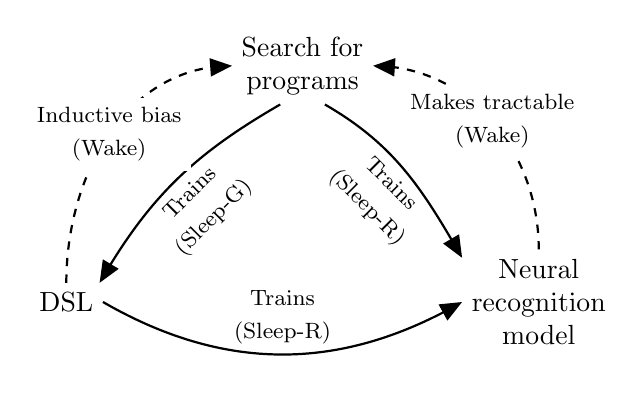
\begin{tikzpicture}
    \begin{scope}[shift = {(1,-1)}]
    \node[align = center](synthesis) at (6,4) {Search for \\programs};
    \node[align = center](DSL) at (3,1) {DSL};
    \node[align = center](recognitionModel) at (9,1) {Neural\\recognition \\model};

    \draw [->,thick] (synthesis.-120) to[out = -150,in = 60] node[below,rotate = 45,align = center]{{\footnotesize Trains}\\{\footnotesize (Sleep-G)}} (DSL.30);
    \draw [->,thick] (synthesis.-60) to[out = -30,in = 120] node[below,rotate=-45,align = center]{{\footnotesize Trains}\\{\footnotesize (Sleep-R)}} (recognitionModel.150);
    \draw [->,thick] (DSL.east) to[out = -30,in = 210] node[above, align = center]{{\footnotesize Trains}\\{\footnotesize (Sleep-R)}} (recognitionModel.west);

    \draw [->,thick,dashed] (DSL.north) to[out = 90,in = 180] node[fill=white,align = center]{  \footnotesize{Inductive bias}\\\footnotesize{(Wake)}} (synthesis.west);
    \draw [->,thick,dashed] (recognitionModel.north) to[out = 90,in = 0] node[fill=white,align = center]{{\footnotesize Makes tractable}\\{\footnotesize (Wake)}} (synthesis.east);
  \end{scope}
    \end{tikzpicture}
  \caption{\system solves for programs, the DSL, and a recognition model. Each of these steps bootstrap off of the others in a Helmholtz-machine inspired wake/sleep inference algorithm.}  \label{feeding}
\end{figure}



\section{Programs that manipulate sequences}\label{sequences}
We apply \system to list processing (Section~\ref{listSection}) and text editing (Section~\ref{textSection}).
For both these domains we use a bidirectional GRU~\cite{cho2014learning} for
the recognition model, and initially provide the system with a generic set
of list processing primitives:
\code{foldr}, \code{unfold}, \code{if}, \code{map}, \code{length},
\code{index}, \code{=}, \code{+}, \code{-}, \code{0}, \code{1}, \code{cons},
\code{car}, \code{cdr}, \code{nil}, and \code{is-nil}.



\subsection{List Processing}\label{listSection}
Synthesizing programs that manipulate data structures is a widely studied
problem in the programming languages community~\cite{feser2015synthesizing}.
%with applications to computer aided programming~\cite{solar2008program}.
We consider this problem within the context of learning functions that
manipulate lists, and which also perform arithmetic operations upon lists of numbers.


\begin{wrapfigure}{r}{0.55\textwidth}\centering
  \begin{tabular}{lll}
    \toprule
    Name & Input & Output \\\midrule
    repeat-2 & [7\, 0] & [7\, 0\, 7\, 0] \\
    drop-3 & [0\, 3\, 8\, 6\, 4] & [6\, 4] \\
    rotate-2 & [8\, 14\, 1\, 9] & [1\, 9\, 8\, 14] \\
    count-head-in-tail & [1\, 2\, 1\, 1\, 3] & 2 \\
    keep-mod-5 & [5\, 9\, 14\, 6\, 3\, 0] & [5\, 0] \\
    product & [7\, 1\, 6\, 2] & 84 \\
    \bottomrule
  \end{tabular}
  \captionof{table}{Some tasks in our list function domain. See the
  supplement for the complete data set.}\label{listexamples}
\end{wrapfigure}
We created 236 human-interpretable list manipulation tasks, each with 15
input/output examples (Tbl.~\ref{listexamples}).
Our data set is interesting in three major ways: many of the tasks require
complex solutions; the tasks were not generated from some latent DSL, and
the agent must learn to solve these complicated problems from only 236
tasks.
Our data set assumes arithmetic operations as well as sequence operations,
so we additionally provide our system with the following arithmetic
primitives: \code{mod}, \code{*}, \code{>}, \code{is-square},
\code{is-prime}.

We evaluated \system on  random 50/50 test/train split.
Interestingly, we found that the recognition model provided little benefit for the training
tasks. However, it yielded faster search times on held out tasks, allowing
more tasks to be solved before timing out.
The system composed 38 new subroutines, yielding a more expressive DSL more closely matching the
domain (left of Tbl.~\ref{initialExampleDSL}, right of
Fig.~\ref{fragmentExample}). See the supplement for a complete list of
DSL primitives discovered by \systemEnding.

\subsection{Text Editing}\label{textSection}
Synthesizing programs that edit text is a classic problem in the
programming languages and AI literatures~\cite{menon2013machine,lau2001programming},
and algorithms that learn text editing programs ship in Microsoft Excel~\cite{gulwani2011automating}.
This prior work presumes a hand-engineered DSL.
We show \system can instead start out with generic sequence manipulation
primitives and recover many of the higher-level building blocks that have
made these other text editing systems successful.

Because our enumerative search procedure cannot generate string
constants, we instead enumerate programs with string-valued
parameters.  For example, to learn a program that prepends ``Dr.'', we
enumerate $\text{\code{(}}f_3\code{ string s)}$ -- where $f_3$ is the
learned appending primitive (Fig.~\ref{initialExampleDSL}) --- and then
define $\probability[x|p]$ by approximately marginalizing out the
string parameters via a simple dynamic program.
In Sec.~\ref{regressionSection}, we will use a similar trick to
synthesize programs containing real numbers, but using gradient
descent instead of dynamic programming.

We trained our system on a corpus of 109 automatically generated text editing tasks, with 4 input/output examples each.
After three iterations, it assembles a DSL containing a dozen new functions (center of Fig.~\ref{initialExampleDSL}) that let it solve 
all of the training tasks.
But, how well does the  learned DSL generalized to real text-editing scenarios?
We tested, but did not train, on the 108 text editing problems from the SyGuS~\cite{alur2016sygus} program synthesis competition. Before any learning,
\system solves 3.7\% of the problems with an average search time of 235 seconds.
After learning,
it solves 74.1\%, and does so much faster,
solving them in an average of 29 seconds.
As of the 2017 SyGuS competition,
the best-performing algorithm solves 79.6\% of the problems.
But, SyGuS comes with a
different hand-engineered DSL \emph{for each text editing problem}.\footnote{SyGuS text editing problems also prespecify the set of allowed string constants for each task. For these experiments, our system did not use this assistance.}
Here  we learned a single DSL
that applied generically to
all of the tasks,
and perform comparably to the best
prior work.

\section{Symbolic Regression: Programs from visual input}\label{regressionSection}
We apply \system
to symbolic regression problems.  Here, the
agent observes points along the curve of a function, and must write a
program that fits those points.  We initially equip our learner with
addition, multiplication, and division, and task it with solving
100 symbolic regression problems, each either a polynomial of degree
1--4 or a rational function.  The recognition model is a
convolutional network that observes an image of the target function's
graph (Fig.~\ref{functions}) --- visually, different kinds of
polynomials and rational functions produce different kinds of graphs,
and so the recognition model can learn to look at a graph and predict
what kind of function best explains it.  A key difficulty, however, is
that these problems are best solved with programs containing real
numbers.  Our solution to this difficulty is to enumerate
 programs with real-valued parameters, and then fit those
parameters by automatically differentiating through the programs the
system writes and use gradient descent to fit the parameters.
We define the likelihood model, $\probability[x|p]$, by assuming a Gaussian noise model for the input/output examples,
and penalize the use of real-valued parameters using the BIC~\cite{Bishop:2006:PRM:1162264}.

\begin{wrapfigure}{r}{0.45\textwidth}\vspace{-0.5cm} \newcommand{\functionSize}{1.5cm}\centering
  
\includegraphics[width = \functionSize]{figures/functions/6.png}
  
\includegraphics[width = \functionSize]{figures/functions/48.png}
  
\includegraphics[width = \functionSize]{figures/functions/102.png}
  
\includegraphics[width = \functionSize]{figures/functions/116.png}\\
  \vspace{1pt}
\includegraphics[width = \functionSize]{figures/functions/181.png}
  
\includegraphics[width = \functionSize]{figures/functions/160.png}
  
\includegraphics[width = \functionSize]{figures/functions/149.png}
    
\includegraphics[width = \functionSize]{figures/functions/187.png}
  \caption{Recognition model input for symbolic regression. DSL learns subroutines for polynomials (top row) and rational functions (bottom row) while the recognition  model jointly learns to look at a graph of the function (above) and predict which of those subroutines best explains the observation.}\label{functions}\vspace{-2cm}
\end{wrapfigure}
\system learns a DSL containing 13 new functions,
most of which are templates for polynomials of different orders or ratios of polynomials.
It also learns to find programs that minimize the number of continuous degrees of freedom.
For example, it learns to represent linear functions with the program
\code{(* real (+ x real))}, which has two continuous degrees of freedom, and represents quartic functions using the invented DSL primitive $f_4$ in the rightmost column of Fig.~\ref{initialExampleDSL}
which has five continuous parameters.
This phenomenon arises from our Bayesian framing --- both the implicit bias towards shorter programs and the likelihood model's BIC penalty.


\section{Quantitative Results}\label{quantitative}

We compare with ablations of our model on held out tasks.
The purpose of this ablation study is 
both to examine the role of each component of \systemEnding,
as well as to compare with
prior approaches in the literature:
a head-to-head
comparison of program synthesizers is complicated by the fact that
each system, including ours, makes idiosyncratic 
assumptions about the space of programs and the statement of tasks.
\begin{wraptable}{r}{0.55\textwidth}
\vspace{-5pt}
%% This radically shrinks the table
\tabcolsep=2.5pt
\renewcommand{\arraystretch}{0.5}
\begin{tabular}{lcccccc}
  \toprule& Ours& 
    No NN & SE&NPS & PCFG & Enum \\
  \midrule
  \multicolumn{7}{c}{\emph{List Processing}}\\
  \midrule
  \% solved&\textbf{79\%}\footnotemark & 
  76\% &71\%&35\%&62\%&37\%\\
  Solve time&  4.1s&5.8s&10.6s&34.7s&43.4s&20.2s\\
  \midrule
  \multicolumn{7}{c}{\emph{Text Editing}}\\
  \midrule
  \% solved&\textbf{74\%} &43\% &30\%&33\%&0\%&4\%\\
  Solve time& 29s&65s&38s&80s&--&235s\\
  \midrule
  \multicolumn{7}{c}{\emph{Symbolic Regression}}\\
  \midrule
  \% solved&   \textbf{84\% }&75\%&62\%&38\%&38\%&37\% \\
  Solve time&  24s& 40s  &28s&31s&55s&29s\\
  \bottomrule
  \end{tabular}
\caption{\% held-out test tasks solved. Solve time: averaged over solved
  tasks.  %SE: NPS: trained like RobustFill/DeepCoder.  PCFG: model w/o
  %structure learning.  Enum: model w/o any learning.  %% MDL:
  %% $-\expect\left[\probability[x|p] \right]$. For domains other than
  %% symbolic regression MDL is 0 nats.
  %% For symbolic regression MDL is a
  %% proxy for \# of continuous parameters.
}\vspace{-0.5cm}\label{baselineComparisons} \end{wraptable}
Nevertheless, much prior work can be modeled within our setup. 
We compare with the following ablations (Tbl~\ref{baselineComparisons};
Fig~\ref{learningCurves}):
\\\noindent \textbf{No NN:} lesions the recognition model.
\\\noindent \textbf{NPS}, which does not learn the DSL,
instead learning the recognition model
from samples drawn from the fixed DSL.
We call this NPS (Neural Program Synthesis)
because this is closest to how
RobustFill~\cite{devlin2017robustfill} and DeepCoder~\cite{balog2016deepcoder} are trained.
\\\noindent \textbf{SE}, which lesions the recognition model and restricts the DSL  learning algorithm to
only add \textbf{S}ub\textbf{E}xpressions of programs in the frontiers to the DSL. This is how most prior approaches have learned libraries of functions~\cite{Dechter:2013:BLV:2540128.2540316,DBLP:conf/icml/LiangJK10,DBLP:conf/ecai/LinDETM14}.
\\\noindent \textbf{PCFG}, which lesions the recognition model and does not learn the DSL,
but instead learns the parameters of the DSL ($\theta$), learning the parameters of a PCFG while not learning any of the structure.
\\\noindent \textbf{Enum}, which enumerates a frontier without any learning --- equivalently, our first search step.
\footnotetext[2]{Due to a last-minute bug we ran the list processing experiments
without training the recognition model on ``Helmholtz machine'' style data. We
are rerunning this experiment and anticipate improved quantitative results for
list processing --- notice the recognition model helps much more for text editing and symbolic regression.} &
%For each domain,
%% We are interested both in how many tasks the
%% agent can solve and how quickly it can find those solutions.
%% Tbl.~\ref{baselineComparisons}
%% compares our model against these alternatives.
%% We consistently
%% improve on the baselines,
%% and find that lesioning the recognition model
%% and lesioning it also slows down the convergence of the algorithm,
%% taking more iterations to reach a given number of tasks solved (Fig.~\ref{learningCurves}).
%% This supports a view of the recognition model as a way of amortizing the cost of search.



\begin{figure}\centering
  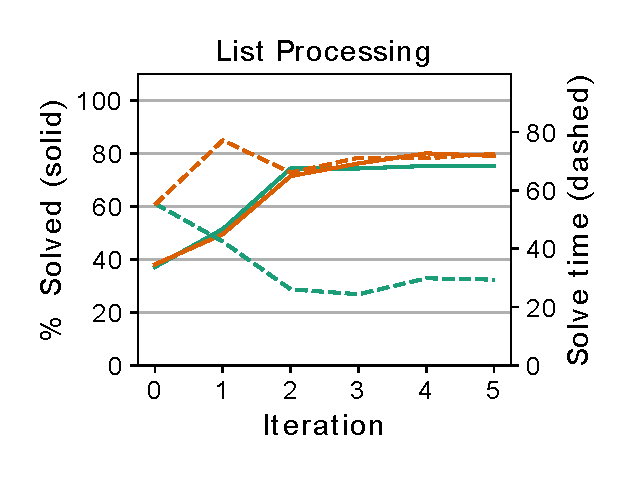
\includegraphics[width = 4.5cm]{figures/listLearningCurve.eps}
  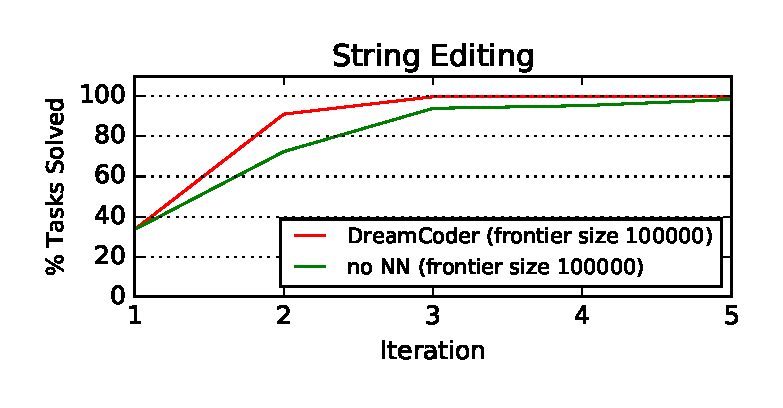
\includegraphics[width = 4.5cm]{figures/textLearningCurve.eps}
  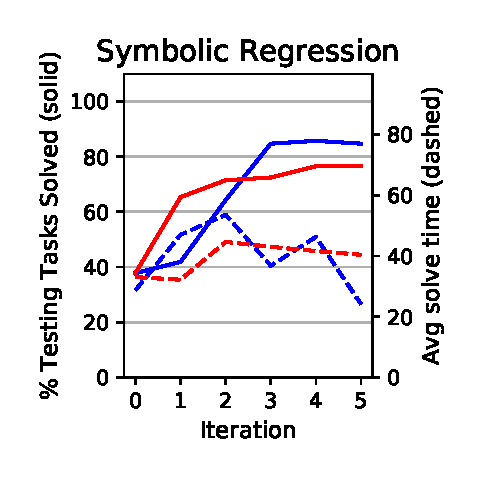
\includegraphics[width = 4.5cm]{figures/rationalCurve.eps}
  \caption{Learning curves for \system both with (\orange{in orange}) and without
  (\teal{in teal}) the recognition model. Solid lines: \% holdout testing tasks solved. Dashed lines: Average solve time.}\label{learningCurves}
\end{figure}

\section{Related Work}
 Our work is far from the first for learning to learn programs,
 an idea that goes back to Solomonoff~\cite{solomonoff1989system}:

 \noindent \textbf{Deep learning:} Much recent work in the ML community has
 focused on creating neural networks that regress from
 input/output examples to programs~\cite{devlin2017robustfill,devlin2017neural,menon2013machine,balog2016deepcoder}. %This family of work is closest to our RF/DC baseline.
\systemEnding's recognition model draws heavily from this line of work, particularly from~\cite{menon2013machine}.
We see these prior works as operating in a different regime: typically, they train with strong supervision (i.e., with annotated ground-truth programs) on massive data sets (i.e., hundreds of millions~\cite{devlin2017robustfill}).
 Our work   considers a weakly-supervised regime where ground truth programs are not provided and
 the agent must learn from at most a few hundred tasks,
 which is facilitated by our ``Helmholtz machine'' style recognition model.%(Sec.~\ref{recognitionSection}).
 
 \noindent \textbf{Inventing new subroutines for program induction:}
 Several program induction algorithms, most prominently the EC algorithm~\cite{Dechter:2013:BLV:2540128.2540316}, take as their goal to learn new, reusable subroutines that are shared in a multitask setting. We find this work inspiring and motivating,
 and extend it along two dimensions: (1) we propose a new algorithm for
 inducing reusable subroutines, based on Fragment Grammars~\cite{tim};
 and (2) we show how to combine these techniques with bottom-up neural recognition models.
 Other instances of this related idea are~\cite{DBLP:conf/icml/LiangJK10}, Schmidhuber's OOPS model~\cite{schmidhuber2004optimal}, and predicate invention in Inductive Logic Programming~\cite{DBLP:conf/ecai/LinDETM14}.
 
\noindent\textbf{Bayesian Program
 Learning:} Our work is an instance of
 Bayesian Program
 Learning (BPL; see~\citep{lake2015human,Dechter:2013:BLV:2540128.2540316,ellis2016sampling,DBLP:conf/icml/LiangJK10}). Previous BPL systems have largely assumed a fixed DSL (but see~\cite{DBLP:conf/icml/LiangJK10}),
 and our contribution here is a general way of doing BPL with less hand-engineering of the DSL.
 
\section{Discussion}

\parbox{0.58\textwidth}{

%\paragraph{Outlook.}
We contribute an algorithm, \systemEnding, that learns to program by
bootstrapping a DSL with new domain-specific primitives that the algorithm
itself discovers, together with a neural recognition model that learns how to
efficiently deploy the DSL on new tasks. We believe this integration of top-down
symbolic representations and bottom-up neural networks --- both of them learned
--- helps make program induction systems more generally useful for AI. Many
directions remain open.
%\paragraph{Future.}
Two immediate goals are to integrate more sophisticated neural recognition
models~\cite{devlin2017robustfill} and program
synthesizers~\cite{solar2008program}, which may improve performance in some
domains over the generic methods used here.
We are in the process of applying our algorithm to generative programs and
prototyped this with a turtle-like domain: Figure~\ref{geomCompiled} gives some
preliminary results for turtle graphics  --- see Section 1 of the supplementary material for more
details.  Another direction is to explore DSL meta-learning: can we find a
\emph{single} universal primitive set that could effectively bootstrap DSLs for
new domains, including the three domains considered,  but also many others?
}\hfill
\begin{minipage}{0.4\textwidth}
  \centering
  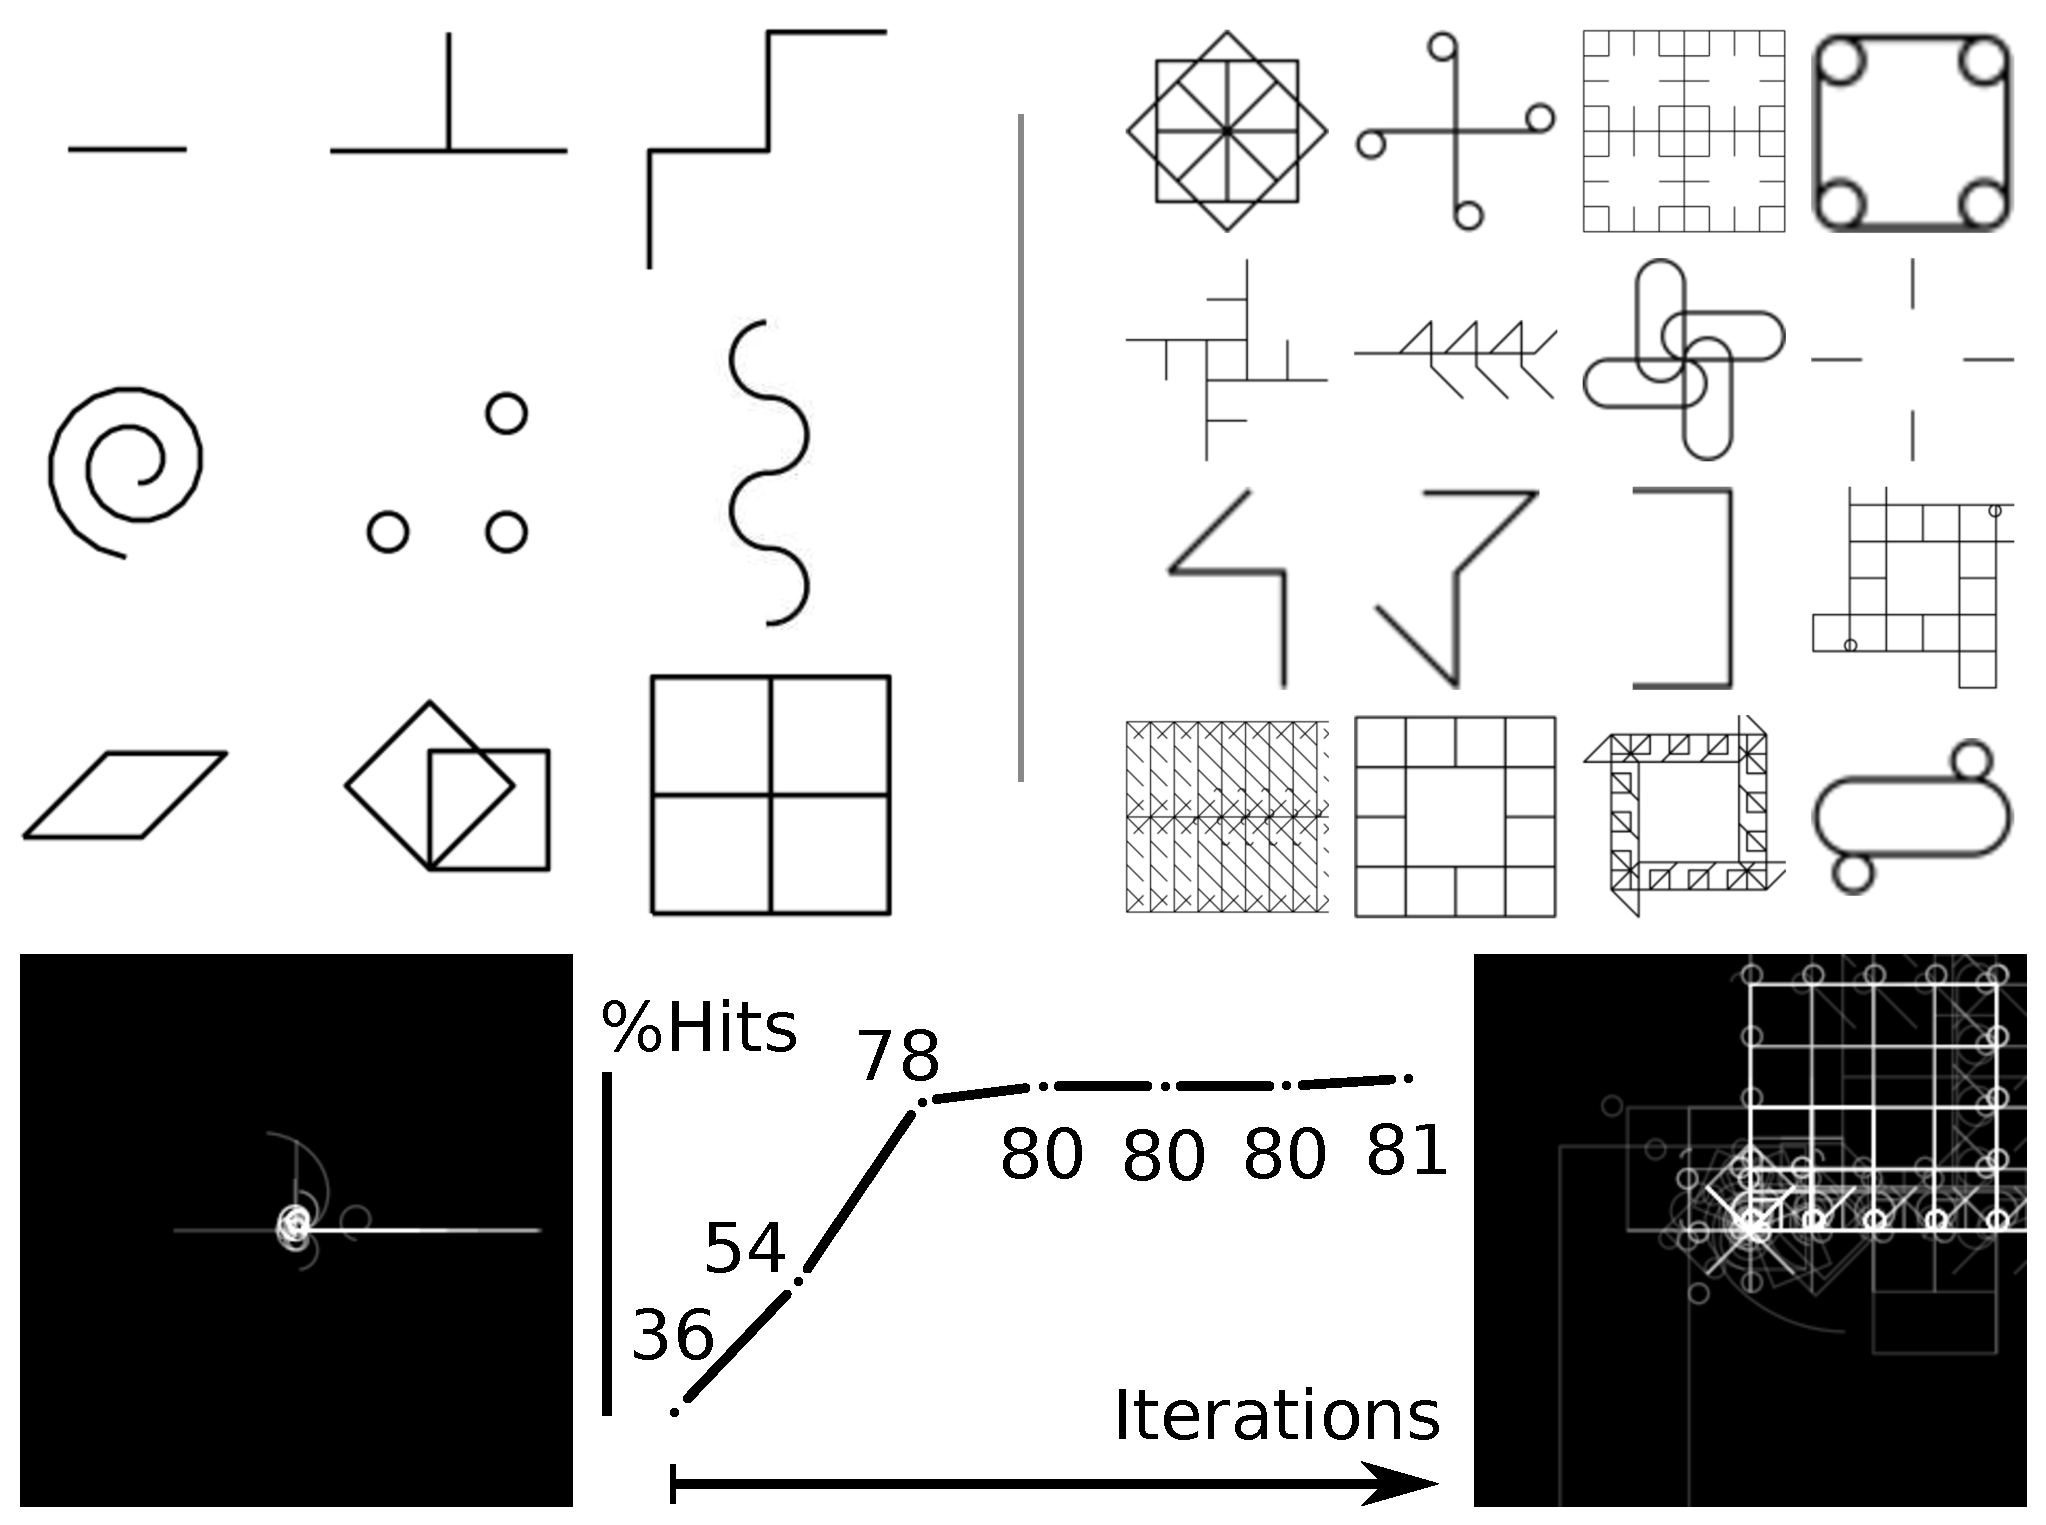
\includegraphics[width=\textwidth]{figures/geomCompiled.eps} 
  \captionof{figure}{
  Top left: Example training tasks. Top right: samples from the learned DSL.
 Bottom: \% holdout testing tasks solved (middle), on sides are the averaged samples from the DSL
  before any training (left) and after last iteration (right).}
\label{geomCompiled}
\end{minipage}

\bibliography{main}
\bibliographystyle{icml2018}
\end{document}
